% Design Development 
\chapter{Design Development}

Tasked with creating the future of flying for disabled passengers, we carried out process-centric and product-centric needfinding and benchmarking to understand our design space. The insights garnered from these explorations led us to the following key insights which are detailed further in Appendix C.  These insights led us to finally focus on both what happens to the passenger and what happens to his/her wheelchair. The following section is here to show the path our team took to get to this design choice.

\section{User needfinding}
Fall quarter was spent primarily focused on needfinding and benchmarking (see Appendix A) in order to get a firm grasp of the problem we were trying to solving. Given that ``redesigning the flying experience for people with reduced mobility" is a huge design space with a great number of possible users, we used our findings to further develop our understanding of the user segment with the biggest need as well as their specific burning need. After looking at countless available products and interviewing a myriad of different users, we decided to focus on wheelchair users as our target user. 

Throughout our interviews we heard many horror stories about mobility in the cabin and how it affected how wheelchair users prepare for their flights (i.e. ensuring they won't have to use the restroom), how they choose to situate themselves during flight (i.e. choosing to sit in the window seat so they won't be in anyone's way) or whether they even choose to fly. Our final ``experience" prototype for Fall Quarter involved the idea of having seats on rails that would automatically adjust width when a person needed to enter or exit a row. This way, the wheelchair user would have more room to get into their seat and would also be able to choose the seat they wanted because the row would shift when someone else needed to get out, freeing the wheelchair user of the guilt of being in the way. This design addressed painpoints we all encounter while flying (moving in a constrained space) yet would significantly improve the experience for our target user. \\

When we started Winter Quarter we came in with a brand new prospective on the project given that we had just acquired 3 new team members. In order to get the most out of it, we started the quarter by multiple brainstorming sessions in order to identify what were the elements of the aircraft we could change to most improve the travel experience for a wheelchair user- the user we had decided to focus on. 

Through these brainstorming sessions we wanted to understand our design space and its limitations. We also wanted to build a strong relationship with our global partners in Brazil and agreed to meet them on Skype at least once a week and share our common work via a Podio web platform. This helped us keep our teams organized ourselves and aware of the other team's progress and allowed us to tackle and learn about different issues during two big steps in our design development: the dark horse and functional prototypes. 

\section{Dark horse}

\subsection{Introduction}
Winter quarter began with the first of three prototyping missions, Dark Horse.  Named after the horse racing term, this prototyping mission fosters the unimaginable and impossible; improbable solutions to the presented problem from Embraer.  The mission called for the brainstorming of out-of-the-box ideas and the  creation of a physical prototype for this seemimngly implausible solutions.  The learning that occurs from the mission is more important in comparison to the actual building process and it is intended to guide the team toward their final vision. 

\subsection{Benchmarking}
During our interviews and needfinding research, we realized carry-on luggage was a huge concern. Currently, luggage is stored in a very burdensome and unintuitive way and with our prototype we sought out to redesign the carry-on luggage experience. 
Our users have voiced their concerns about not being able to store/reach their luggage as well as the panic they feel when they are not aware of where their belongings are being stored. Our team looked at a couple of different designs out there that use the vertical space within the airplane in a different manner to accommodate both people and luggage in a more user friendly way. 

\begin{figure}[h]
  \centering
     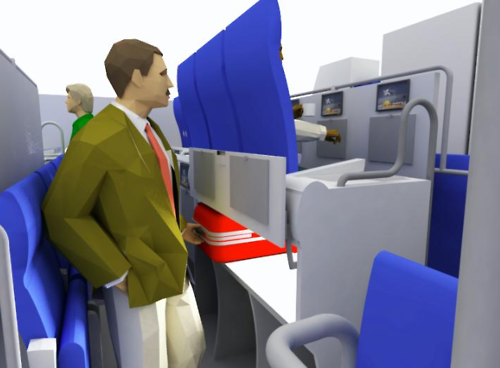
\includegraphics[width=7cm]{images/luggage_trays.png}
   \caption{Design that allows for easier luggage storage for all passengers Source: http://www.gizmag.com/future-of-air-travel-comfortable-seating/17751/}
  \label{fig:luggage_trays.png}
\end{figure}  

The design shown in Figure \ref{fig:luggage_trays.png} displays a cabin layout where consecutive rows of seats are on different levels, allowing passengers to store their luggage behind their tray but under the seat of the person in front of them. This design puts luggage at the ideal height for both standing and sitting passengers as depicted by the image in Figure \ref{fig:correct_height.png}, a standard design rule for accessibility and mobility.  

\begin{figure}[h]
  \centering
     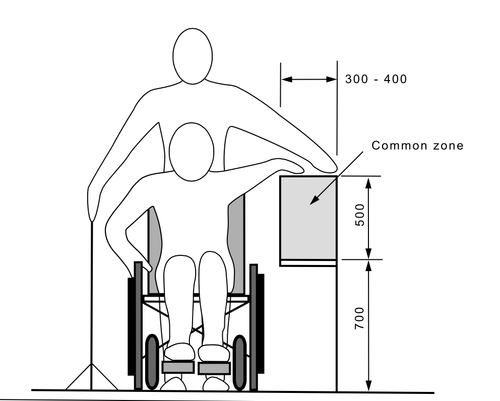
\includegraphics[width=7cm]{images/correct_height.png}
   \caption{Ideal height for reaching objects for both sitting and standing passengers. Source: https://law.resource.org/pub/nz/ibr/nzs.4121.2001.svg.html}
  \label{fig:correct_height.png}
\end{figure} 

Another design solution we explored was actually having two seats on top of each other as shown in Figure \ref{fig:vertical_with_luggage.jpg}. This design opens up the area under the stairs for luggage storage, which could also include a passenger’s wheelchair, allowing for a less stressful flying experience for handicapped users. The bed next to the seat could also be used to provide passengers flying with toddlers with extra room to put them in so that they do not have to sit on their lap throughout the whole flight. 

\begin{figure}[h]
  \centering
     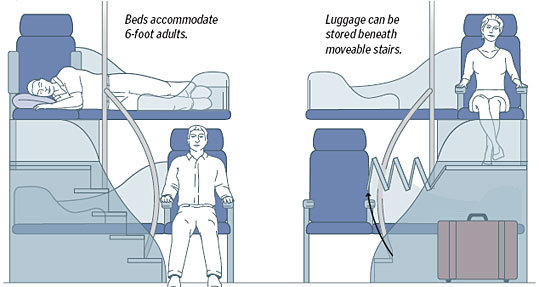
\includegraphics[width=7cm]{images/vertical_with_luggage.jpg}
   \caption{Vertical cabin configuration with luggage storage} % Source: http://www.boston.com/business/articles/2009/06/15/taking_airline_seat_configurations_vertical}
  \label{fig:vertical_with_luggage.jpg}
\end{figure} 

This benchmarking really brought to light the lack on control disabled passengers feel over their belongings. Since they already suffer from mobility constraints, they are not able to fully control where their belongings are stored which causes a huge amount of anxiety. We realized later on that this anxiety was only increased when the object in question wasn't just a bag but rather a mobility device. 


Another main concern for our user was the actual transfer process and how they would get from an aisle chair to their seat. We know that today people can use transfer boards, they can be carried by someone else or, if they are strong enough, they can attempt to transfer themselves(although the limited space in the cabin makes this virtually  impossible). We found that there are some products on the market utilized in analogous situations that could make the transfer experience better, such as the “harness” shown in Figure \ref{fig:harness.jpg} or the walker in Figure \ref{fig:walker.jpg}. We believed that the walker would be an interesting solution if we were able to add mechanisms that would lower the bar supporting the person’s weight to get it closer to the seat and that would swing the blue supports open such that the person would come in contact with the chair. In the end, we decided to opt for a more futuristic vision and decided to widen the airplane aisle and get rid of the transfer all together. 

\begin{figure}[h]
  \centering
     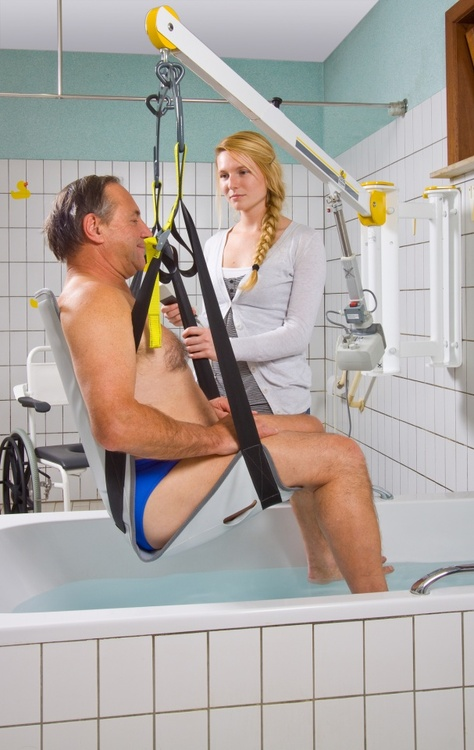
\includegraphics[scale=0.3]{images/harness.jpg}
   \caption{Harness used to get disabled out of the bath.}% Source: http://www.handimove.com/en/products/bath-seat-pvc/}
  \label{fig:harness.jpg}
\end{figure} 


\begin{figure}[h]
  \centering
     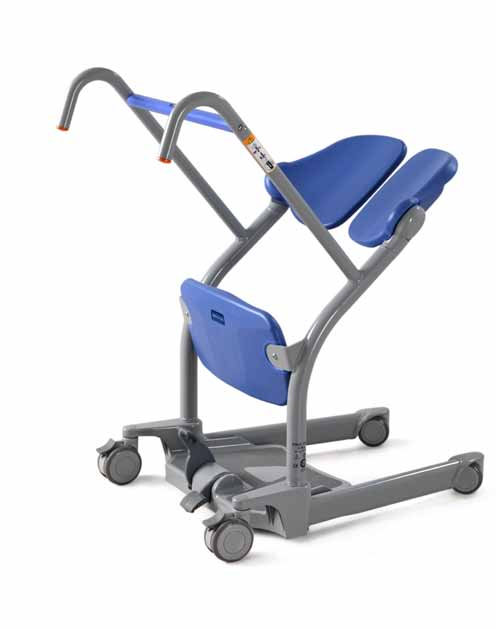
\includegraphics[scale=0.5]{images/walker.jpg}
   \caption{Walker that could be adapted to become a better aisle chair.}% Source: http://mobilityexpress.com/Sara-Stedy-Seated-Transfer-Device_1154.htm}
  \label{fig:walker.jpg}
\end{figure} 

\subsection{Description of the prototype}
Currently, people with reduced mobility have to first transfer from their own wheelchair to an uncomfortable and narrow aisle wheelchair. Once boarding starts, the user is brought to his/her seat by a flight attendant or an airline employee and is then transferred to his/her seat, usually by being carried over their shoulders. This process is long, dehumazing and it deprives them from their independence. Since the boarding process is such a pain point for our users, we decided to tackle this problem to improve their experience and give them more independence. Our team thought that if we could enable people with reduced mobility to enter the aircraft with their own wheelchair and then give them the possibility to transfer themselves from their wheelchair to their seat without someone else helping them it would considerably improve their experience.
\\

%During the boarding process the two steps that are critical for our users are :

 %\begin{easylist}[itemize]

%& First, the access to their seats. 

%& Second, the luggage storage. People with reduced mobility frequently cannot access the luggage compartment because it is too high, so our team thought that if we could imagine a system that makes the luggage compartment go up and down by just pressing a button it would also contribute to make the flight experience better for people with reduced mobility.

%\end{easylist}


\textbf{Helping our user access his/her seat :}

Our objective was to enable passengers to enter the aircraft with their own wheelchair and to do so we had to figure out a way to make the aisle wider. Initially we did not want to take into account the constraint of keeping the number of seats in the aircraft the same so we imagined a new cabin layout for boarding. The idea was to have the aisle seats on rails so that they could be moved and lined up with the window seats as shown in Figure \ref{fig:first_new_cabin_layout} . 

\begin{figure}[h]
  \centering
     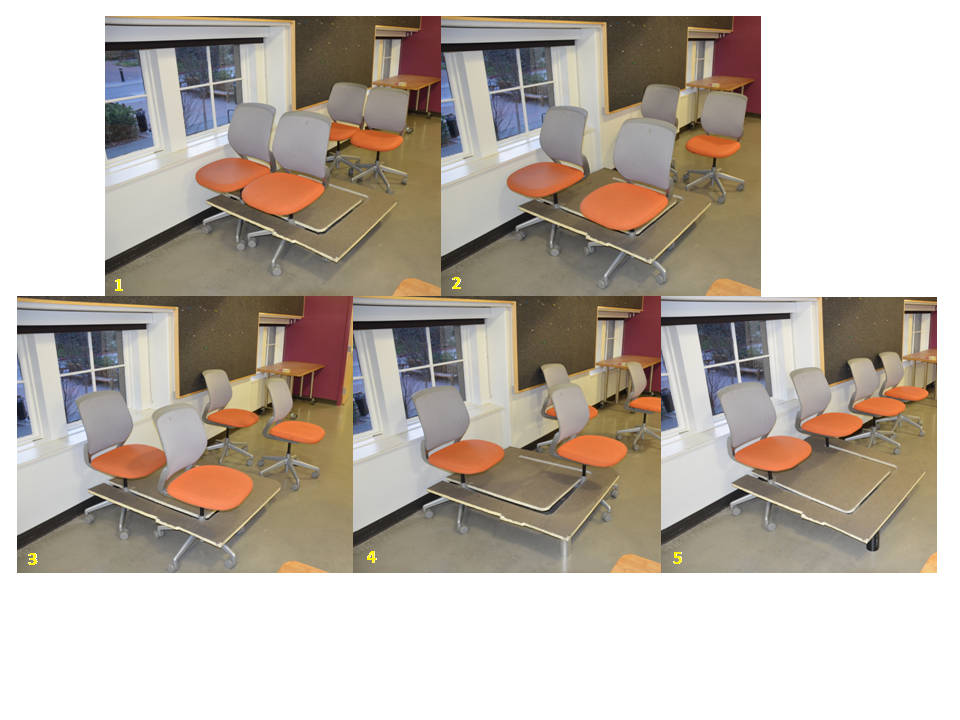
\includegraphics[width=7cm]{images/first_new_cabin_layout.png}
   \caption{Our first new cabin layout for boarding the plane}
  \label{fig:first_new_cabin_layout}
\end{figure} 

With this system, all the seats would be lined up on each side of the plane and the aisle during the boarding process would therefore be three times bigger than during the flight, giving people with reduced mobility the ability to enter the aircraft with their own wheelchair since the average width of a wheelchair (30’’ as shown in Figure \ref{fig:wheelchair_dimensions} ), would now fit down the bigger aisle. 

\begin{figure}[h]
  \centering
     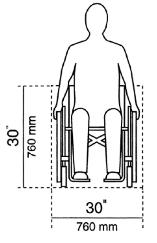
\includegraphics[scale=1]{images/wheelchair_dimensions.png}
   \caption{Standard wheelchair dimensions}
  \label{fig:wheelchair_dimensions}
\end{figure}

But we realized that with this system it would be impossible to keep the total number of passengers on board the aircraft the same since the proposed boarding layout required too much space per seat. 

Therefore, we thought of a second cabin layout for the boarding process which would also make the aisle wider but in a more reasonable way. We looked at the dimensions of a standard Embraer plane (Figure \ref{fig:embraer_plane} ) and found out that if we were able to angle the rows by 46.2° (see Figure \ref{fig:angled_seats}) from their current position we could make the aisle wide enough (42.87’’) to enable our passengers to reach their seats in their own wheelchair while still keeping the total number of seats the same.

\begin{figure}[h]
  \centering
     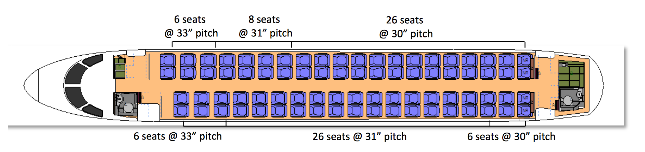
\includegraphics[width=7cm]{images/embraer_plane.png}
   \caption{Standard Embraer plane cabin layout}
  \label{fig:embraer_plane}
\end{figure}

Our concept was to initially have all of the rows of the plane linked to a mechanism that would rotate the seats before the boarding process, making a wider aisle for passengers. Passengers with reduced mobility who have reached their seats with their own wheelchair would be able to transfer themselves  to their plane seats. 
\begin{figure}[h]
  \centering
     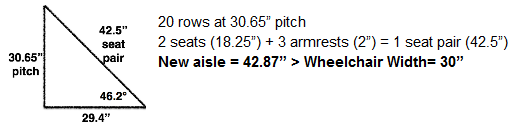
\includegraphics[width=7cm]{images/angled_seats.png}
   \caption{New cabin layout with angled seats for boarding}
  \label{fig:angled_seats}
\end{figure}

Once the passengers are all seated (potentially while the aircraft is taxiing towards the runway) the seats would go back to the standard non-angled cabin configuration for take-off and would remain in that state for the duration of the flight. When the plane stops at the gate and is ready for passengers to disembark, the seats would be angled again and flight attendants would bring passengers with reduced mobility their own wheelchair. This configuration would completely remove the need for an aisle wheelchair.\\ 


%\textbf{2. Helping our user accessing the luggage compartment :}

%We found out that accessing the seat is not the only problem disabled people are confronted with: they also have a big issue when they want to store their personal items in the luggage compartment. In order to fix this, our team designed a luggage compartment that can go up and down on demand, controlled by our user pressing a button (Figure \ref{fig:embraer_plane}).

%\begin{figure}[h]
%  \centering
%     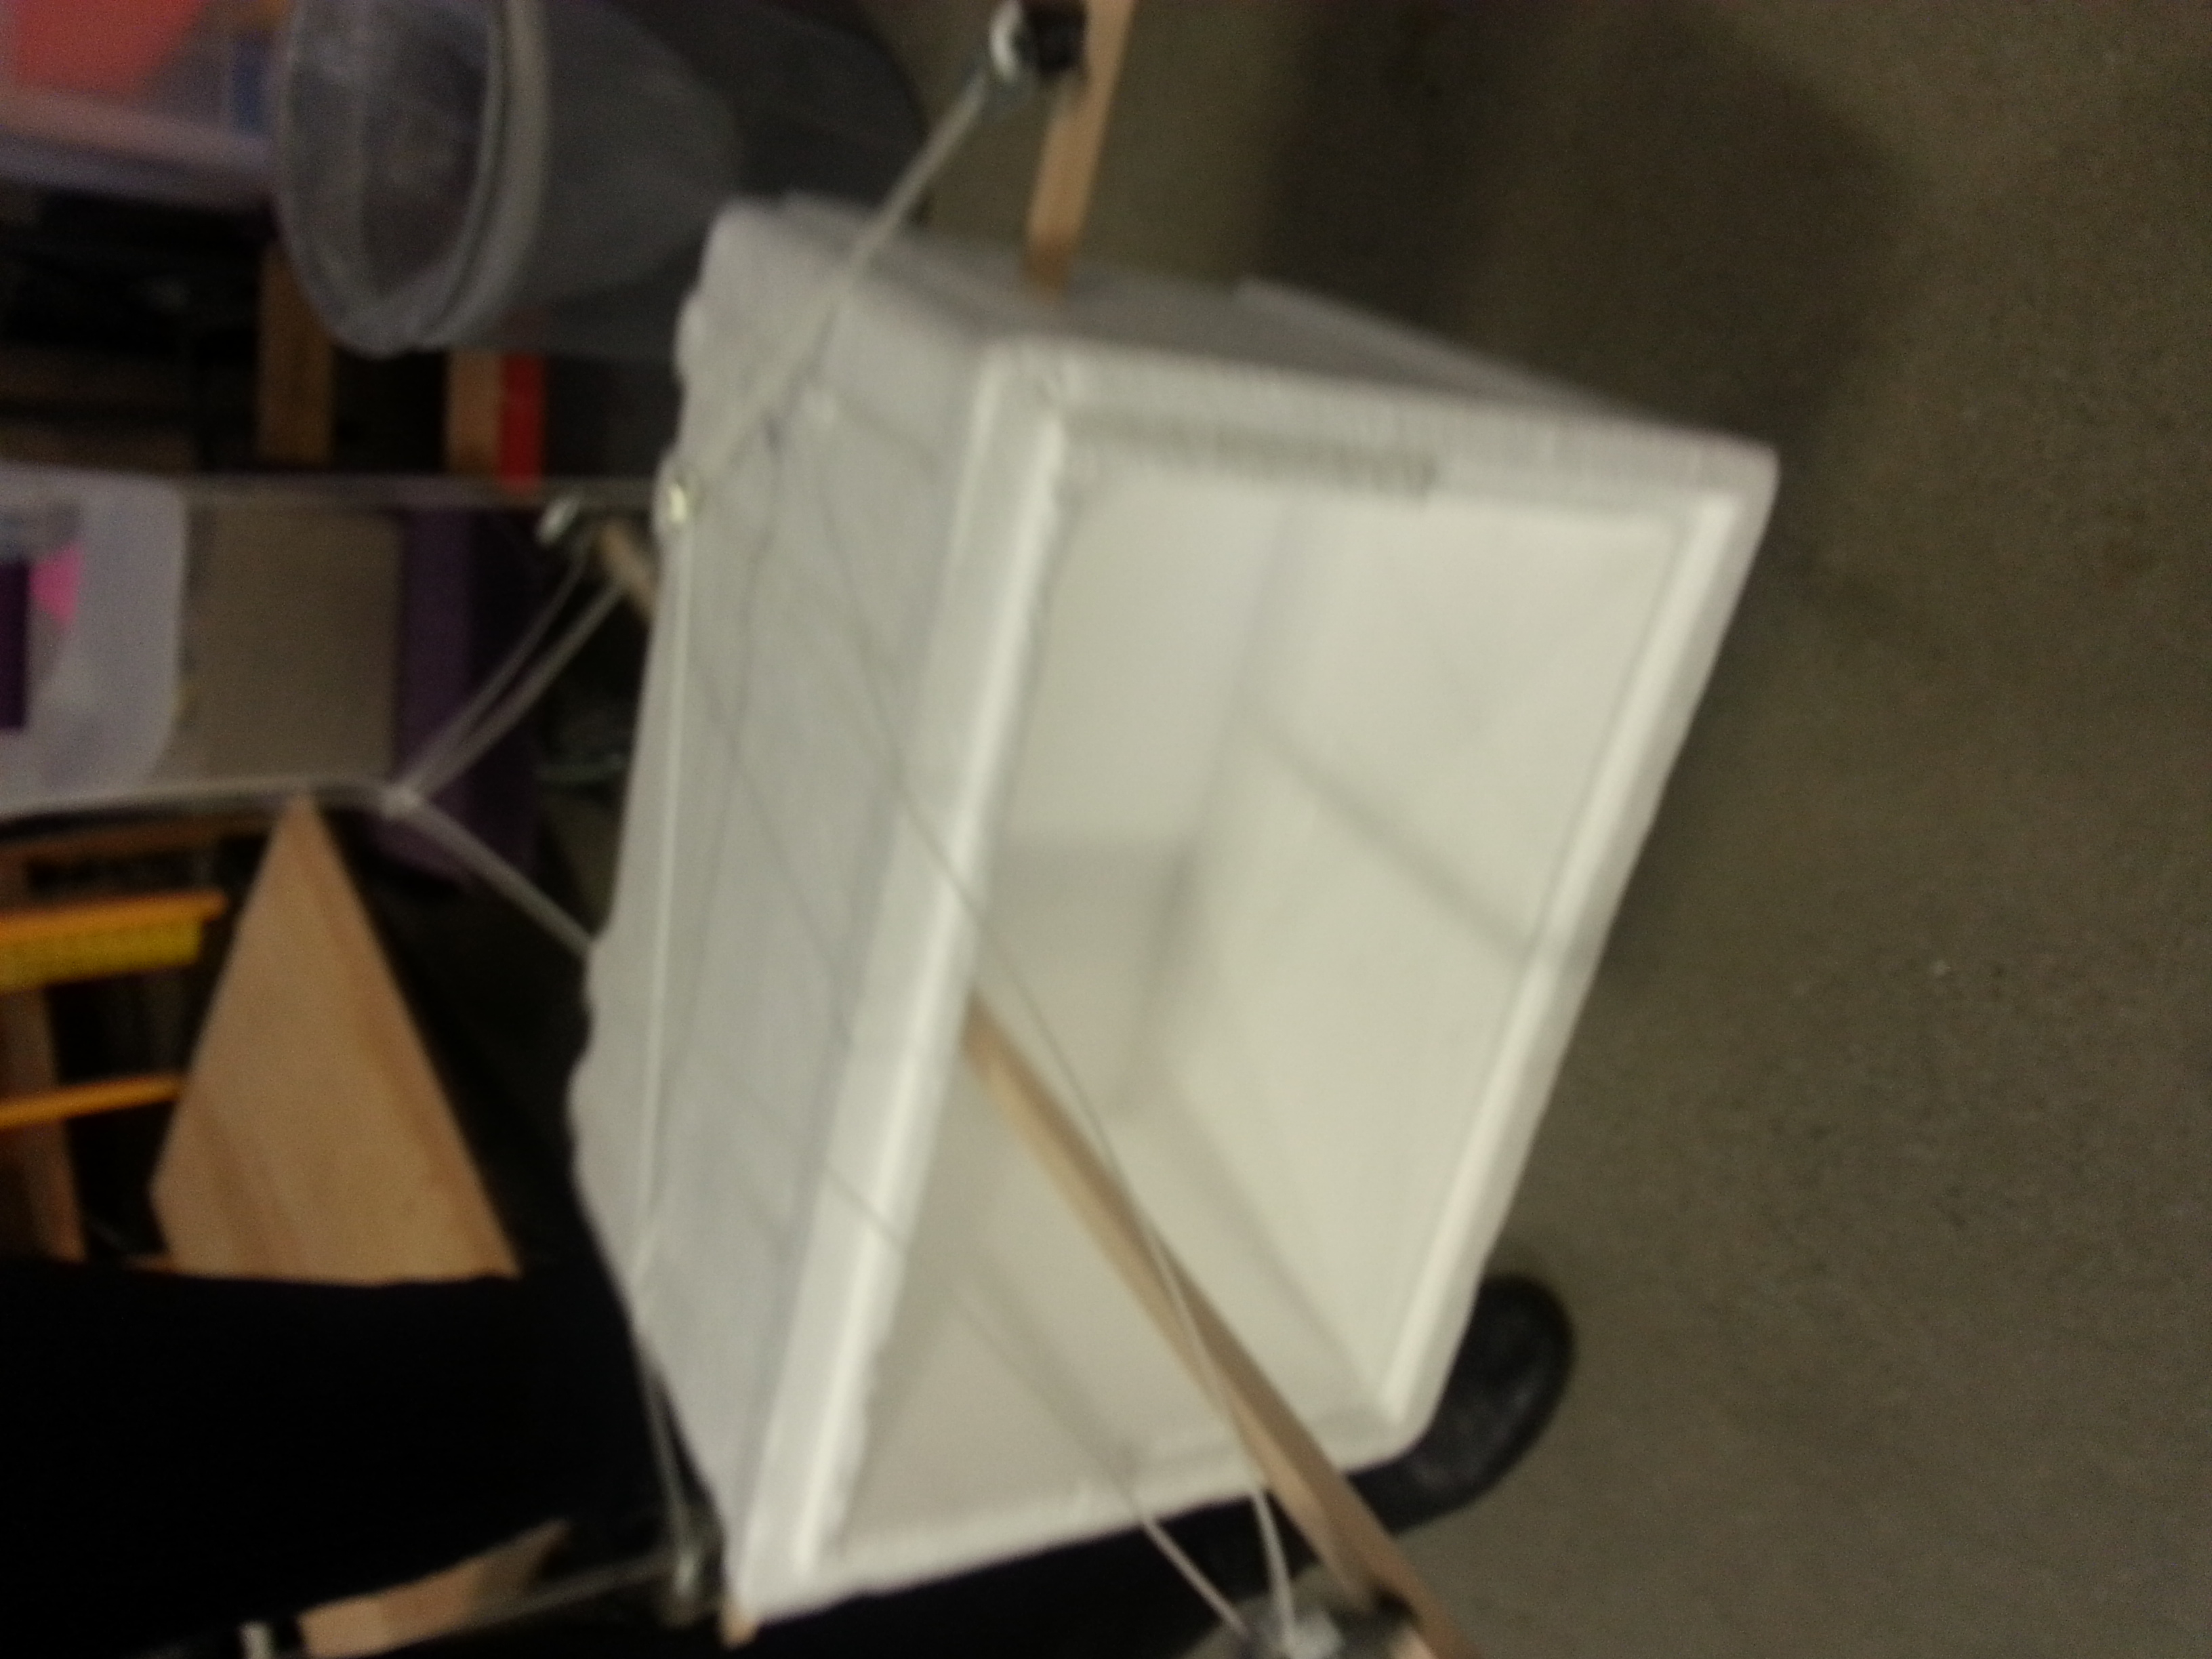
\includegraphics[width=7cm]{images/20140130_170818.jpg}
%  \caption{Our luggage compartment which is accessible on demand by pressing a button}
%  \label{fig:our_luggage_compartment}
%\end{figure}

%In order to build this system we designed a mechanism made of rope and pulleys that is inspired from systems used to stabilize cameras that are mounted on drones and model aircraft. While piloting the system that causes the camera to move, the device has to remain stable. This mechanism avoids the creation of moments that could cause the ropes to tangle and knot. For our system we wanted to have a luggage compartment that does not experience torques and that can come up and down in the most smooth and stable way.

\subsection{Learnings}
Several classmates and peers were users for this prototype and provided the majority of our learnings.  However, some of the learnings came directly from team observations during user testing. 
\\

\textbf{Reconfiguration:}
\begin{easylist}[itemize]
	& Our testing revealed that the users were concerned about what would happen to their feet during the transformation of angled seating to the regular configuration and vice versa.  Some users suggested the addition of a footrest.  But where would the ideal location be? This revelation is very important to our target users because some of them do not have the ability to move their legs out of the way or to move with the chair.  This would also mean they would have to manually put their feet on a footrest, and the ideal position of the footrest would need to be designed to help the target users have a better experience.
	& A single, continuous rotation mechanism would be better than multiple discrete ones for all passengers.  The users commented that the mechanism should be similar to the movement of a car seat because it so slow it is barely felt. In addition, the window seat felt like it experienced less movement partly because the displacement was smaller than for the aisle seat.  This is important due to the benchmarking findings of last quarter that showed that the target users preferred the window seat over the aisle seat. 
	& Passengers would be able to board faster due to a wider aisle that allows for easier maneuvering of the cabin space.  The wider aisle would allow for a double line of traffic to head down the aisle instead of one line. 
	& The wider aisle would allow for a wheelchair to be able to maneuver down the aisle to the seat.  The wheelchair would have space on both sides as it moves down the aisle to allow for a comfortable fit.  It would be easier for a mobility challenged passenger to get into the aisle seat but they may need a handle to access the window. 
	& The legroom is the limiting factor with the reconfiguration.  When the seats are in the angled arrangement, the window seats have less legroom than in the normal configuration.  The angle of the seats would need to be reconfigured to allow for a smaller angle with more legroom but still create a wider aisle with plenty of tolerance for a wheelchair. However, it was noted that it is easier to board and deboard with angled seats.  Thus, angled seats would be the preferred configuration for boarding and disembarking from the plane. 
	& It may be possible to achieve the desired effect by only rotating several of the aisle seats, allowing increased access to those seats specifically.

\end{easylist}


%\textbf{Luggage storage:}
%\begin{easylist}[itemize]
%	& The luggage bin needs to move with the seats into the angled configurations. With the bins situated parallel to the normal cabin configuration when the seats are angled, it is difficult to load the luggage into the bin without awkward movements. 
%	& The luggage bin should be lowered to arm level instead of head or face level.  Users felt claustrophobic when the bin was at head level due to the reduction in vision. The bin was in the line of sight which made it uncomfortable and a very closed-off space.  
%	& The bin should have a door and have a slightly steeper angle or have a lip. Luggage moves during flight due to turbulence and shifting due flight. This would prevent luggage falling out on the passengers or items being broken. 
%	& A more rigid lowering mechanism needs to be used instead of the string and rope mechanism that was used during prototyping.  Users did not feel that the bin was stable and looked scared as it was lowered down.  They feared the bin might move during lowering, raising, or turbulence causing it to hit them or bring their belongings.  
%	& More research for optimal lowering position needs to be conducted.  The position that we prototyped did not receive good feedback from the users.  Therefore, several iterations need to be performed to see what would be best for our target users and other passengers
%	& Most of the users wanted to store luggage before they sat in their seat.  The orientation of the bin and the height of the bin makes this a very awkward and uncomfortable task.  When the users sat with their luggage, they felt that they were crowded and did not know what to do with the luggage until the bin was available.  The mechanism to raise and lower the bin needs to be fast and stable to allow for ease of access to the seat and aisle depending on the activity.
%\end{easylist}

\section{Going Back to The Need}

Following the wrap up of our prototypes, the team decided to take a step back to figure out if we were truly solving the burning need. We analyzed all of our prototypes up to this point and saw an overarching theme we were trying to address: giving our users their independence back. With independence as our umbrella, our team looked at the whole flying experience piece by piece (see Appendix B), with the purpose of identifying the points at which independence truly breaks down. 

We went back to our needfinding from fall quarter, sent surveys to both old and new contacts and carried out more interviews. All of these allowed us to confirm that mobility within the cabin is, in fact, a huge issue. However, this new information also brought to light a burning need we had initially discarded fall quarter - wheelchair storage. Furthermore, both of these needs stem from the same procedure the wheelchair user is forced to go through: that of giving up his/her wheelchair. \\

\textbf{The Problem}

Imagine you are a wheelchair user. You arrive at your gate, ready to board your plane, and are told you need to hand over your wheelchair for storage in the cargo hold. At this point, you ask yourself two questions: 
\begin{enumerate}
	\item How will you move now that you don't have your mobility device? 
	\item Will your mobility device arrive safe and sound at your destination?
\end{enumerate}
The following sections will detail the user quotes and research that led us to choosing both of these directions.  
\\

\textbf{Mobility In the Cabin}

In order to confirm the need for improving mobility inside the cabin, we asked our contacts to fill out a survey that would give us a better idea of what exactly would be the most helpful for them. The full survey responses can be found in Appendix D.
 
When asked about the prospect of having an ``on demand"  powered aisle chair, users were keen on the independence it would provide as it would allow them to ``board the plane at [their] own pace and go to the restroom when [they] please." One of our respondants stated that such a device would allow them to ``feel like a passenger for a change and not a sack of coffee beans". This quote clearly depicts the struggle users currently go through when they give up their mobility device and along with it, their independence.

Our team assumed that having such a chair would be a great improvement to the experience yet we could not figure out if the chair had to be completely autonomous and show up on demand or if a flight attendant could bring it to the user. What we found is that users would much rather have automated systems than feel the guilt of inconveniencing someone else to do something for them, even if it only meant they had to bring them a chair just like they bring any passenger a drink or snack. 

Finally, we decided to delve deeper into the transfer process. One of our interviewees, Scott Rains, had told us about a friend who was injured as he was being transferred from the aisle chair into his airplane seat. The airport personnel did not lift him up high enough and his bottom was hit against the armrest. Given that wheelchair users have thinner and more sensitive skin in this area, this caused him lots of pain and even resulted in 3 weeks spent at the hospital. While injuries are not the norm, it is a very dehumanizing and undignified experience, just as Esther Appleyard-Fox states in her tweet in Figure \ref{fig:MobilityTweet.png}. 


\begin{figure}[h]
  \centering
     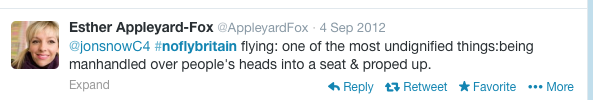
\includegraphics[width=9cm]{images/MobilityTweet.png}
   \caption{Tweet from Esther Appleyard-Fox explaining how she feels when she is transferred when she flies. }
  \label{fig:MobilityTweet.png}
\end{figure}


\textbf{Wheelchair Storage}

As we were looking for more data to substantiate our claim that mobility in the cabin was, in fact, the problem to solve, we stumbled upon another huge problem. During our interview with Aubrie Lee, a student in Product Design at Stanford University who is also a wheelchair user, she mentioned that while mobility inside the cabin is a problem, it is such a short part of her experience that she hardly remembers it as being painful. Part of this is due to the fact that when she travels with her dad he carries her down the aisle which can be more a comforting bonding moment than dehumanizing. However, she emphasized that``the most emotional part of [her] flying experience is having to give up [her] chair and waiting for them to give it back." For her, giving up her chair is ``a huge source of anxiety - as soon as it is out of [her] sight, [she doesn't] know where it is", whether it is going to come back to her unharmed or whether it is even going to make it to her destination. 

In order to understand what can happen to a mobility device on during its transfer to the plane and once in flight, we interviewed an Air France employee working at Toulouse-Balgnac airport (France). All the details form this interview are in Appendix E. It shows how airlines handle wheelchairs from the jetway to the cargo hold and gives some insight on the type of damage that can occur.

A study by Trailblazers \ref{(http://www.mdctrailblazers.org/assets/0000/8262/Trailblazers_AirlineReport_WEB.pdf)}, a group of disabled campaigners across the UK who tackle social issues affecting young disabled people, shows that 60\% of wheelchairs are damaged when traveling with an airline. As David Gillon says in Figure \ref{fig:60percenttweet.png} below, we must do better. 


\begin{figure}[h]
  \centering
     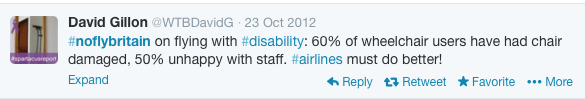
\includegraphics[width=9cm]{images/60percenttweet.png}
   \caption{Tweet from David Gillon on Trailblazers study that shows 60\% of wheelchairs are broken in airline travel. }
  \label{fig:60percenttweet.png}
\end{figure}

\begin{figure}[h]
  \centering
     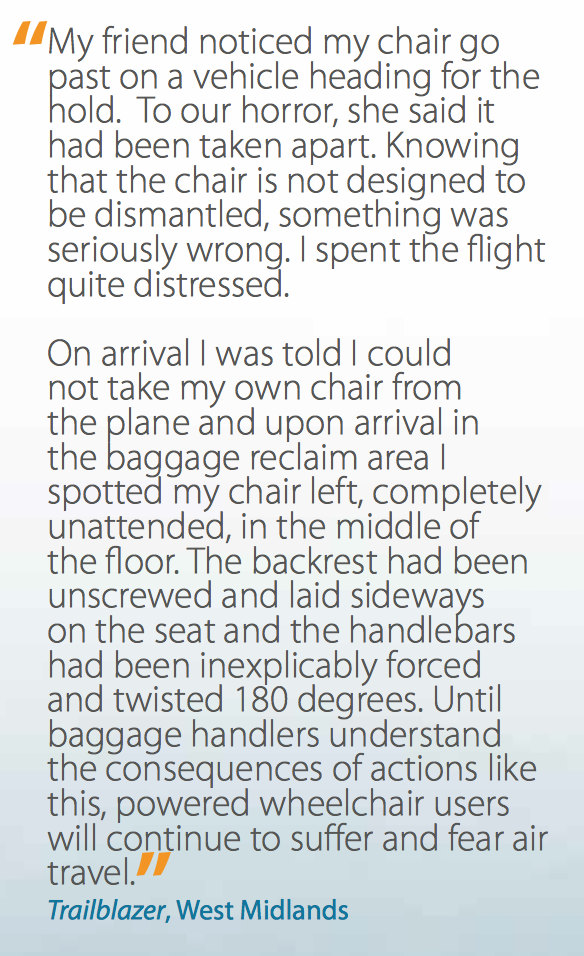
\includegraphics[width=5cm]{images/wheelchairstory.png}
   \caption{Anecdote from a Trailblazer that had her wheelchair broken during flight.}
  \label{fig:wheelchairstory.png}
\end{figure}

Stories like the one shown in Figure \ref{fig:wheelchairstory.png} are not uncommon, with wheelchairs ending up like the one in Figure \ref{fig:brokenwheelchair.png} due to airport personnel attempting to dismantle it or from the wheelchair moving around in the cargo hold. 


\begin{figure}[h]
  \centering
     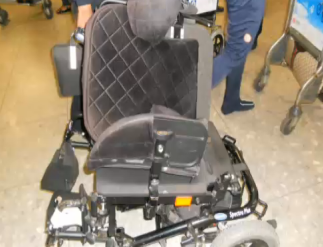
\includegraphics[width=7cm]{images/brokenwheelchair.png}
   \caption{Picture of a broken wheelchair after a flight.}
  \label{fig:brokenwheelchair.png}
\end{figure}

There are also instances of the wheelchair not even making it to the destination, just like what happened to Josie shown in Figure \ref{fig:leftwheelchair.png}. 

\begin{figure}[h]
  \centering
     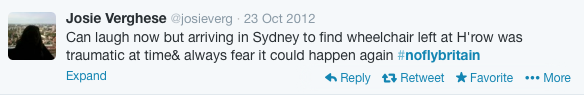
\includegraphics[width=9cm]{images/leftwheelchair.png}
   \caption{Tweet from Josie Verguese about her experience when her wheelchair did not make it to her destination.}
  \label{fig:leftwheelchair.png}
\end{figure}

Now to put this into perspective, imagine that you are a wheelchair user and you rely on your mobility device for you independence. This wheelchair isn't just an object, it is your legs, your independence, part of who you are. As Aubrie stated  my wheelchair``is in limbo between being a physical object and half of me." Now imagine that after your flight, you no longer have the ability to move. This is a HUGE problem for our users, one we need to focus on. \\
\\

 Through  the user interviews, surveys and research depicted above, we have proven to ourselves, our advisors and our users that these are the 2 most compelling needs we need to address for our users and we decided to focus on both for the Functional Prototype. 


\section{Functional Prototype}
The final prototyping mission during Winter Quarter was the Functional Prototype in which we had to create a working prototype with system integrations using materials that could be present in a final vision. The functional mission leads the team into the Spring Quarter by aiding in the finalization of the vision and creating an actionable direction.  To find the direction and the vision, more needfinding might have to take place to confirm a need and verify the thinking and decisions of the team. The Functional mission serves as the stepping point from iterative prototyping missions to the iterative final product mission.

\subsection{Wheelchair Storage Benchmarking}
Before prototyping our first wheelchair storage device we executed a larger search both for existing wheelchair storage and protection devices as well as methods for securing wheelchairs. We found several relevant patents for protection devices as well as regulations for securement, relating primarily to bus travel. \\

\noindent\textbf{Securement}\\
The United States Department of Transportation's Federal Motor Carrier Safety Administration publishes a wide array of regulations. Included amongst the regulations governing school bus safety, Federal Motor Vehicle Safety Standards \textsection 571.222 \cite{fmvs222}, are a number of requirements for how wheelchairs must be secured while in transit. The section requires that the wheelchair is secured in four locations, with an additional three point mounting required to secure the student. Similar topics are covered in further regulations, such as Title 49 \textsection 38.23 \cite{ecfr}. Figure \ref{fig:tie-down} demonstrates the general setup. \\

\begin{figure}[h]
  \centering
     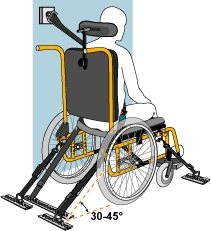
\includegraphics[width=7cm]{images/wc_van.jpg}
   \caption{Wheelchair tie-down setup for van travel}
  \label{fig:tie-down}
\end{figure}

\noindent\textbf{Storage}\\
A group at Utah State University performed market research \cite{USU_survey} and designed a prototype wheelchair storage container, determining that over 50\% of their surveyed users might be or would be interested in their device. A drawing of their box, which provides several securement methods for wheelchairs and other objects, can be seen in Figure \ref{fig:USU_box}; more information is in US Patent application 12/142,662.\cite{USU_patent}

\begin{figure}[h]
  \centering
     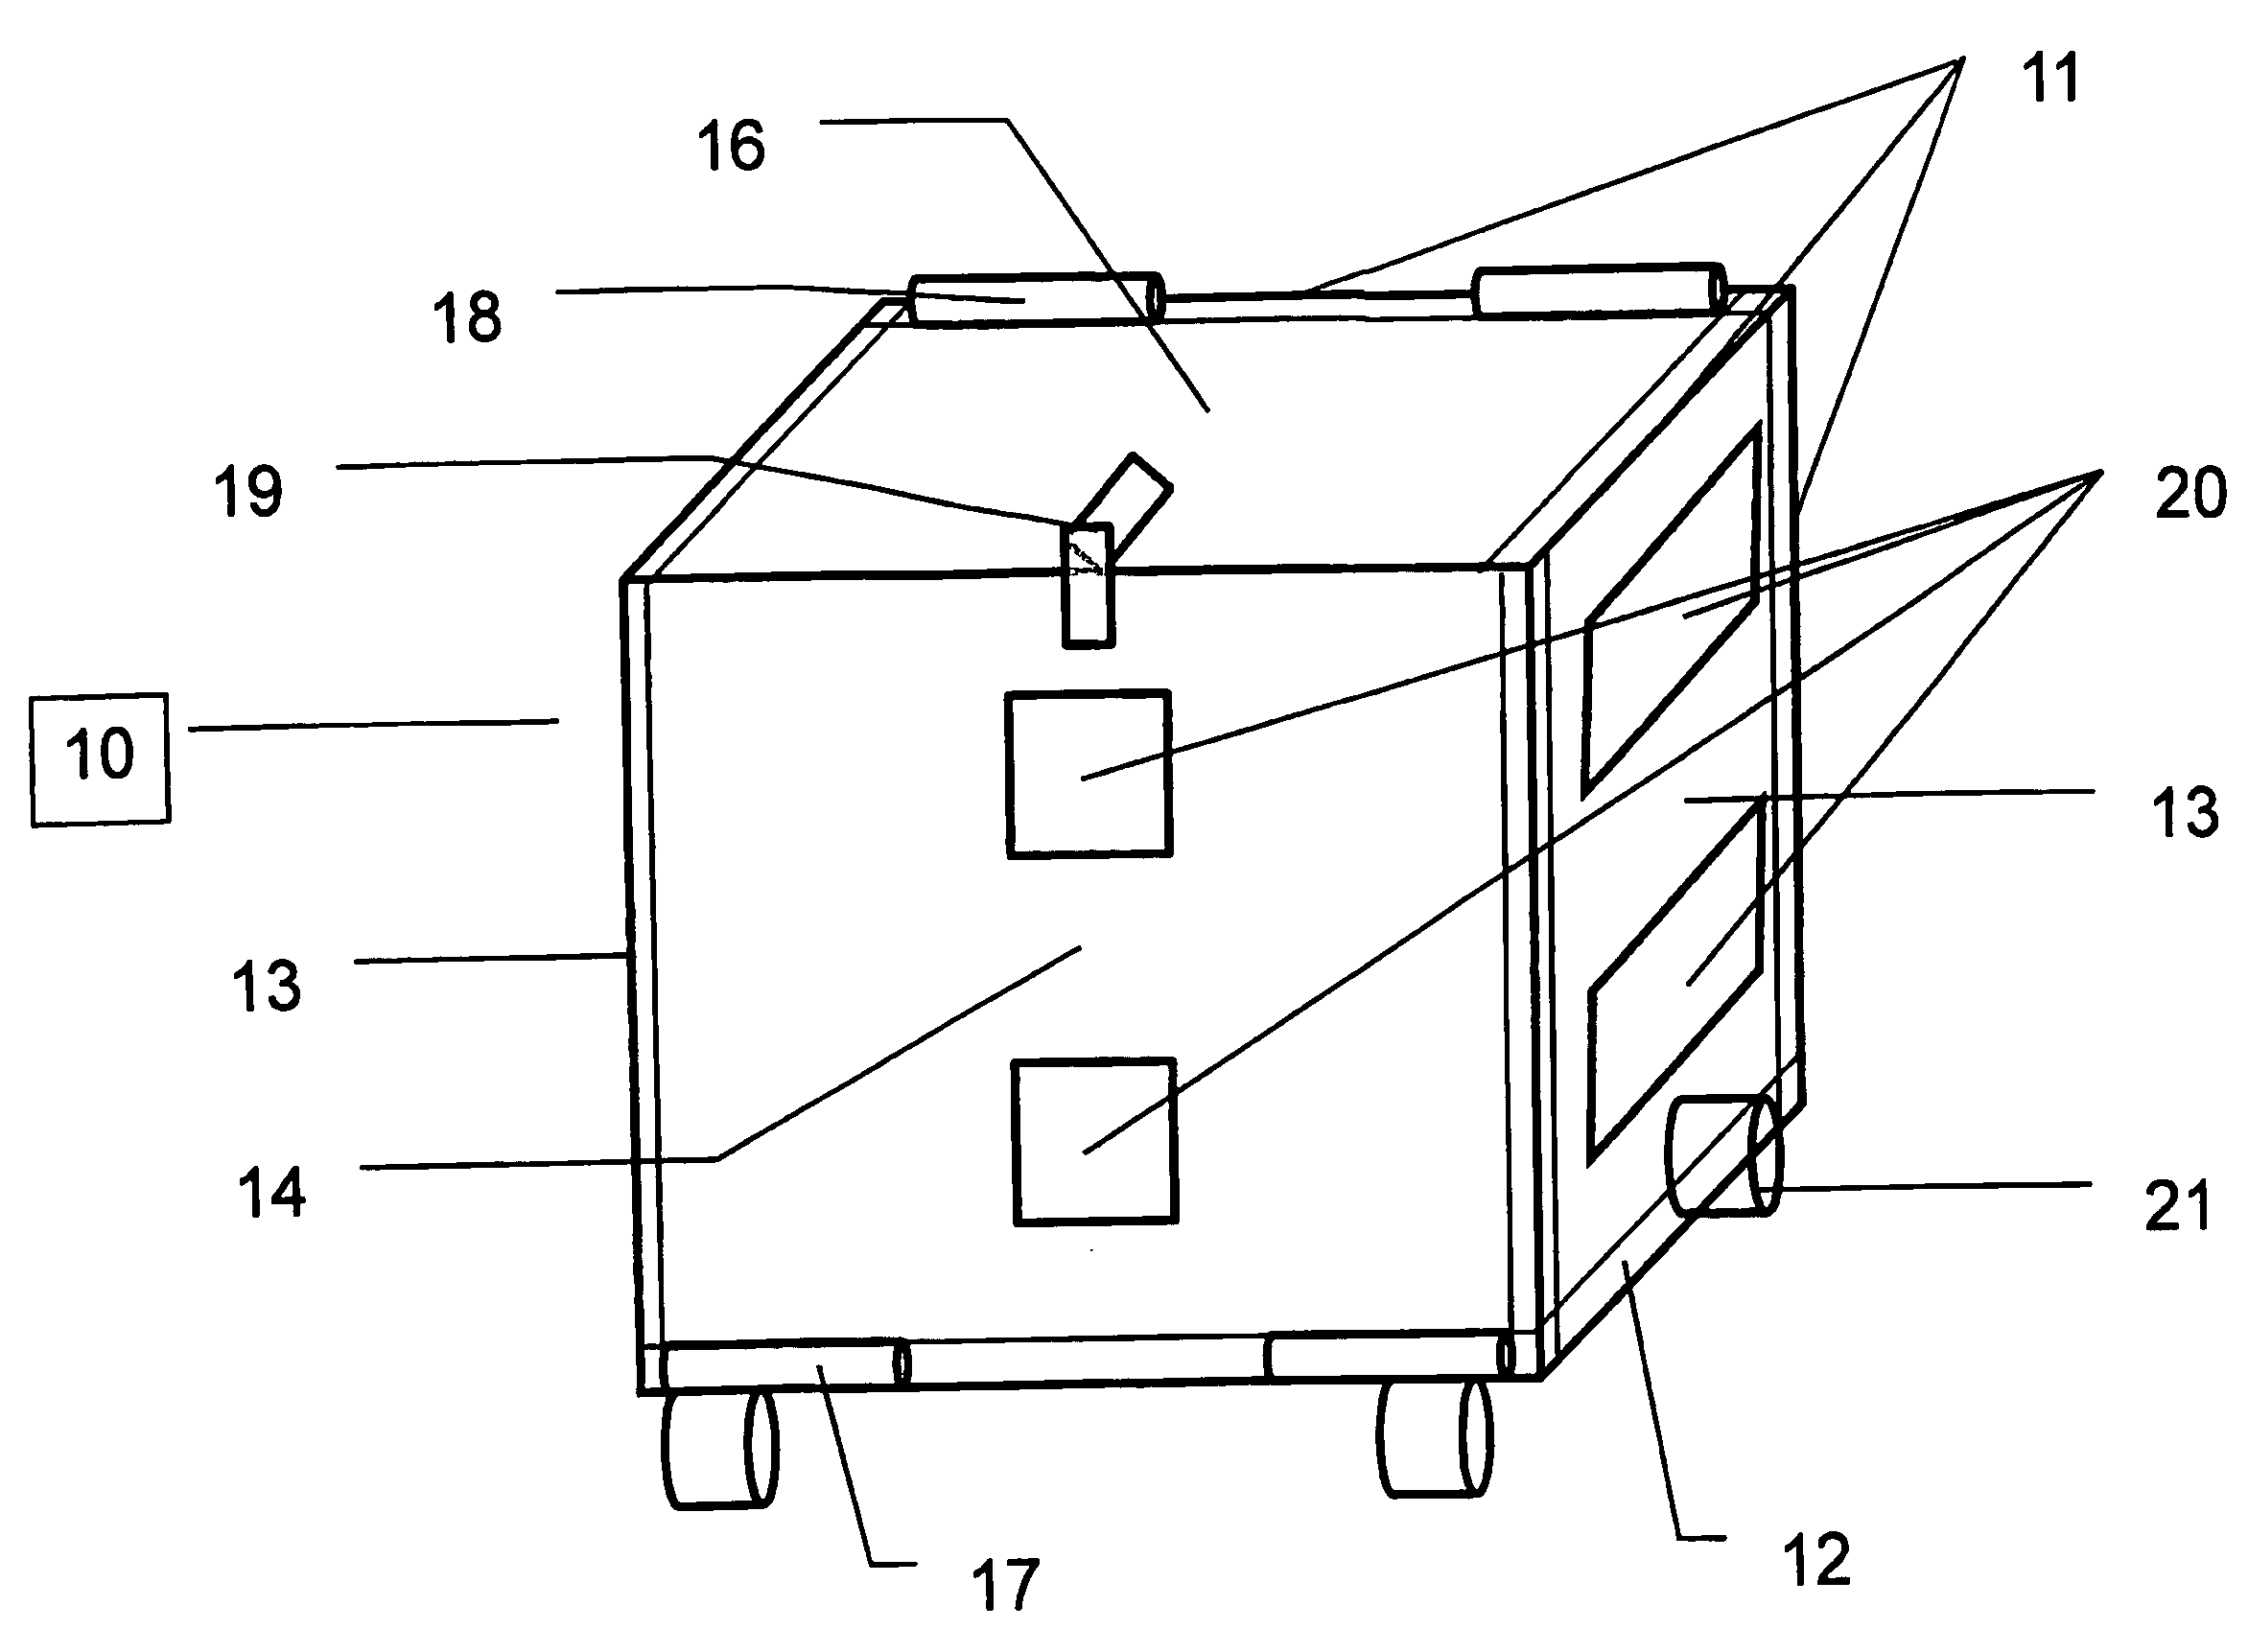
\includegraphics[width=7cm]{images/USU_box.png}
   \caption{Storage container}
  \label{fig:USU_box}
\end{figure}


\subsection{Wheelchair Storage Description}

As our last round of needfinding and research had brought to light the importance of wheelchair storage, the Stanford team decided to prototype the first version of what a wheelchair storage device could look like. This first prototype, shown in 
Figure \ref{fig:wheelchairprototype1.png}, focused on having a rigid floor to distribute the weight of the wheelchair as well as a place to attach the hooks that would secure the wheelchair down. It had rigid walls that would serve to protect the wheelchair (as if it were a box) that were also hinged at the side so they could be moved out of the way as the handler was tying down the wheelchair. We opted to use the straps and hooks mechanism that people are already familiar with from buses and trains to create a sense of trust and security. 

\begin{figure}[h]
  \centering
     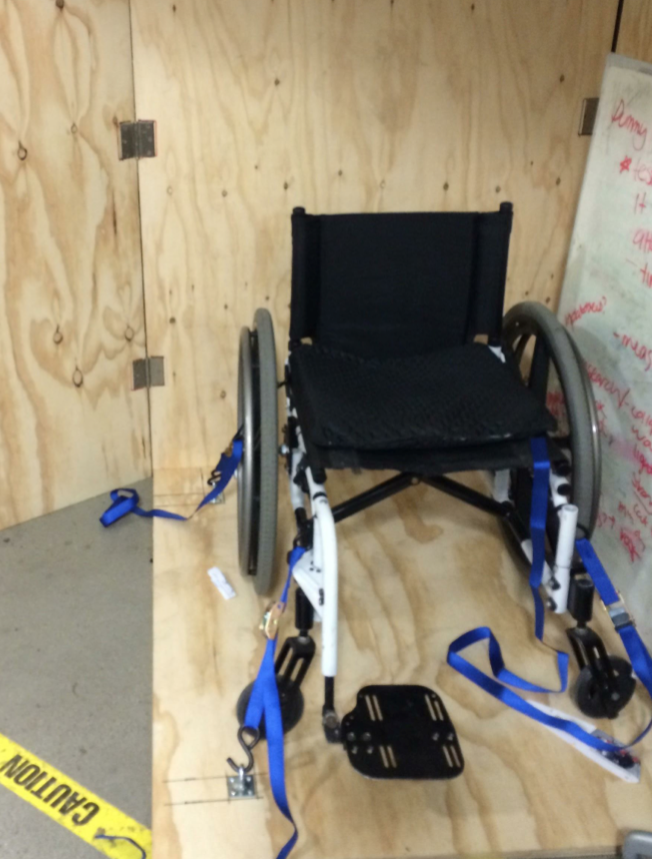
\includegraphics[width=7cm]{images/wheelchairprototype1.png}
   \caption{First prototype of wheelchair storage device.}
  \label{fig:wheelchairprototype1.png}
\end{figure}

Since many of the stories we encountered about wheelchairs being damaged involved airport personnel attempting to disasemble them or handling them poorly, we wanted the wheelchair owner to be present during the securing process, just like they are on a bus or train. This way, the wheelchair user could help the airport personnel speed up the process by providing information about their specific wheelchair and how it should be secured as well as ensure that the airport personnel is not accidentally mishandling their mobility device. At the end of the securing procedure, the container is to be closed up, giving the user satisfaction in knowing that their wheelchair is secure and will arrive safely at their destination. 
 
Because the wheelchair user is present while their wheelchair is secured, we must also enable an easy transfer from their personal wheelchair onto the aisle chair. As shown in the rendering  Figure \ref{fig:storagetransfer.png}, right now this is accomplished by bringing the transfer chair close to the passenger's chair that is already secured. This further explains our use of hinged walls and puts a hard constraint on our system- in order for the wheelchair user to be able to easily transfer once their wheelchair is secured, there must be a way to ``remove'' all walls during securing and ``reappear'' them once the wheelchair is stored for the wheelchair to be protected.

\begin{figure}[h]
  \centering
     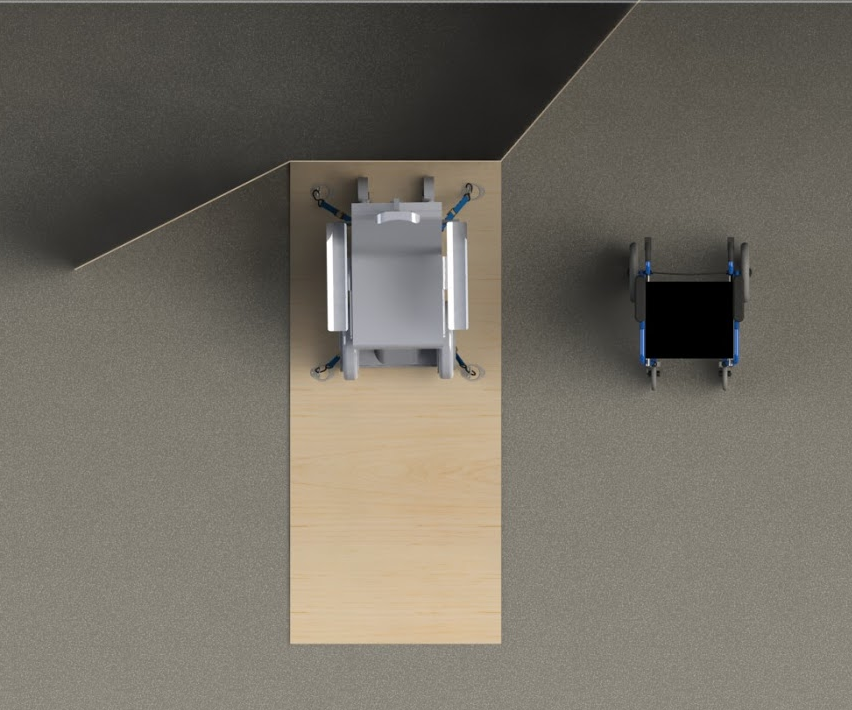
\includegraphics[width=7cm]{images/storagetransfer.png}
   \caption{Rendering of wheelchair and aisle chair side by side once wheelchair has been secured.}
  \label{fig:storagetransfer.png}
\end{figure}

While there are certain hard constraints that were not met with this protoype, we are keeping them in mind and will insitute them in future iterations. We know the container must protect the wheelchair but also fit through the door to the cargo hold as well as fit inside the cargo hold. It needs to be movable, as the wheelchair storage container must travel from the jetway down into the cargo hold. This product must help the luggage handler create a connection with the wheelchair user and gain empathy for the importance of the mobility device that is in their hands; the more important they know it is, the better they will treat it. Finally, the storage device must be lightweight as this is of utmost importance to Embraer and the airlines they serve.

\subsection{Wheelchair Storage Learnings \& Next Steps}

From our first prototype we were able to learn a myriad of things. Primarily, we realized that using a mechanism that wheelchair users are already familiar with is a huge plus; it provides them with a feeling of trust and security that their wheelchair will not be damaged throughout their flight. Thus, we suceeded at providing the user peace of mind with this device. However, we realized it is pretty difficult to line the chair up in the correct configuration in between the protruding hooks that strap the wheelchair to the platform and thus it would be best to have the hooks be flush against the top of the base so they didn't get in the way of the wheelchair manuevering.
We had several users go through the process of securing the wheelchair and found that having simple straps and hooks can be confusing and time consuming. Thus, it is best to have retractable hooks that come out of the base so that the tension is automatically set, making the job of the securer much easier. 

For a process that takes place prior to a flight, time efficiency is extremely important. Airport personnel are very crunched for time as they cannot afford to have any process delay the flight and push their schedules back. This means having very clear instructions for both the wheelchair user as to what's expected of them, where to park and how the process will unfold, as well as for the person securing the wheelchair. For the wheelchair user, we are thinking of ways to transfer this imformation prior to their flight, knowing that most disabled passengers keenly do their research before flying. Having a video that shows the whole process would allow the wheelchair user to be prepared to tell the securer exactly what the right attachment points are and how to best secure the wheelchair down. On the other hand, it is important for the securer to know the correct order of the procedure which can be accomplished by numbers next to each hook as shown in Figure \ref{fig:instructionsstorage.png} and simple drawings depicting what's next. 

\begin{figure}[h]
  \centering
     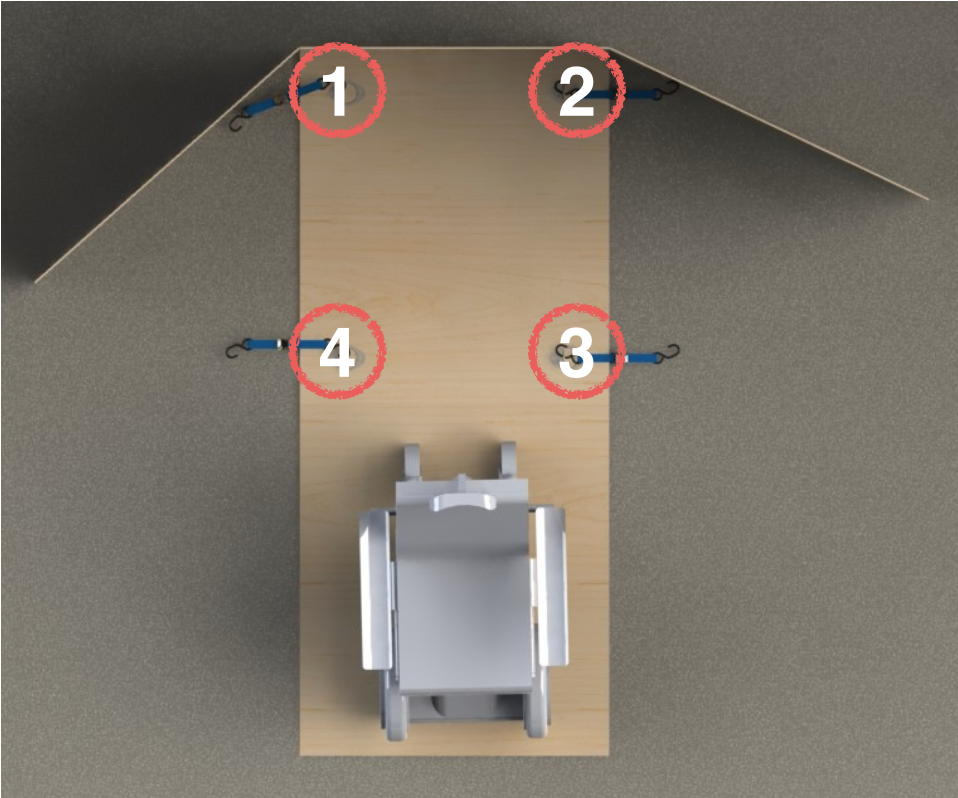
\includegraphics[width=7cm]{images/instructionsstorage.png}
   \caption{Securing the wheelchair}
  \label{fig:instructionsstorage.png}
\end{figure}

Finally, our user testing confirmed our theory that we would need retractable walls. Not only were they necessary for the user to easily transfer onto the aisle chair but they also made the securing process much easier. The back wall, however, was still rigidly attached. This, we found, was not ideal as it made the two hooks in the back extremely hard to reach. With this information in mind, we have been brainstorming different design ideas that would enable for the walls to be completely out of the way during boarding and securing yet would be present during flight to protect the wheelchair from being damaged. We have thought about accordion or telescoping walls as well as having inflatable walls. We really liked the idea of inflatable walls as it provided the wheelchair with protection from damage yet could be blown up to accomodate different types of wheelchair sizes and would be extremely light weight. A preliminary mock up of a possible vision can be seen in Figure \ref{fig:inflatablesrendering.png} With this in mind, we began a feasibility study to understand how possible the use of inflatables would be in the application. 


\begin{figure}[h]
  \centering
     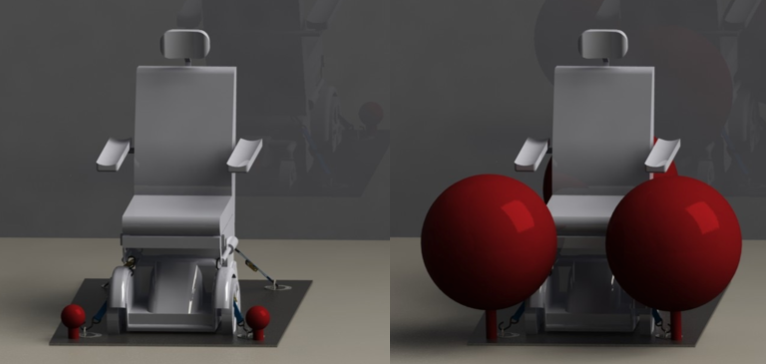
\includegraphics[width=7cm]{images/inflatablesrendering.png}
   \caption{Rendering of a preliminary idea of what an inflatable ``wall'' could be.}
  \label{fig:inflatablesrendering.png}
\end{figure}

%take it from here robbie!

\subsubsection{Inflatable Materials}

In order to test the feasibility of an inflatable device in the cargo hold there were a few problems that needed to be addressed.\\
\noindent\textbf{Pressure}\\
The cargo hold of many planes is not pressurized in order to save on costs. One of our goals was to determine if an inflatable device to protect the wheelchair would pose a problem in low pressure situations. Initially we were unsure as to what the pressure in the cargo hold would be, and as such decided to design for the worst case when the pressure is the same inside the cargo hold as outside. 

It was important to design for this case as regardless of the pressure in the cargo hold, in any emergency situations where the cabin lost power, we would not want any problems to arise in the cargo hold potentially making the situation worse.\\

\noindent\textbf{Temperature}\\
A second potential problem with an inflatable device in the cargo hold is that the luggage does not require the same heating and insulation as passengers. While it may not get as cold as the air outside (approximately -40 C) in normal situations, we must design the device to work reliably even in case of an emergency. \\

\noindent\textbf{Testing}\\
While it may  be possible to test the effects of pressure on an inflatable device without taking it into a plane by increasing the pressure inside the inflatable device (since the pressure differential is the most important aspect to test), its much more difficult to test this pressure differential at a realistic temperature on the ground. Instead we decided it would be best to get an inflatable structure up to approximately the height of a plane and determine what failure modes, if any, would be present. 

In order to do this we attached a fully blown-up arm flotation device to a weather balloon. This balloon was released in order to take the device into the upper atmosphere where it would experience similar conditions to those of an airplane. While it ignores some effects from the natural plane insulation, its a more extreme environment in all cases so its a good measure of feasibility. \\

\noindent\textbf{Results}\\
Unfortunately the barometer which was being used as an altimeter for this experiment failed, and as such we were unable to get reliable altitude data on the flight. However by looking at the videos returned from the launch, and given the group's prior experience with weather balloons, a reasonably reliable estimate of 50,000 - 60,000 ft can be estimated for when the flotation device popped,an altitude which is significantly higher than an Embraer jet flies (37,000 ft maximum). We were able to see small water droplets on the larger weather balloon which froze at high altitudes forming ice crystals.

This experiment showed us that an inflatable solution would in fact be feasible if it was something we wanted to pursue.

\subsubsection{Wheelchair Tracking Concept}

We didn't just want to stop at protecting the wheelchair, we also wanted to give the wheelchair user information regarding their wheelchair. 
We envision a wheelchair tracking system in which each storage container has a unique identifier, such as a QR code, which can be tracked as the container moves from the jetway to the tarmac, into the cargo hold, and then back out again after landing. The identifier can be recognized at a series of checkpoints, which need to consist only of a webcam if a QR code is used. Such a system will provide our users with the peace of mind that their mobility device has not been mistreated or left behind.

\begin{figure}[h!]
  \centering
     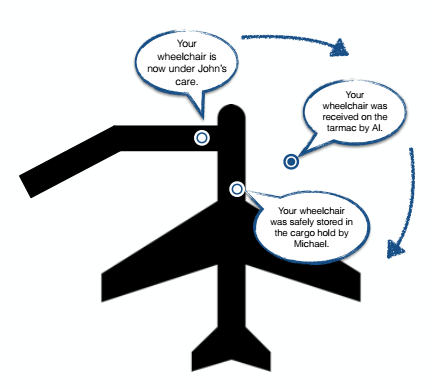
\includegraphics[width=12cm]{images/tracking.png}
   \caption{Wheelchair tracking system overview.}
  \label{fig:tracking}
\end{figure}


An important aspect of this system is that it can also help develop empathy on the part of the baggage handlers. Wheelchair users will have the opportunity to tip handlers who've done a good job in managing their mobility device, both providing an incentive for doing a better job while also helping form a closer connection between two people who may never meet face to face.

An overview of the system and one potential user interaction are in Figures \ref{fig:tracking} and \ref{fig:tips}.


\begin{figure}[h]
  \centering
     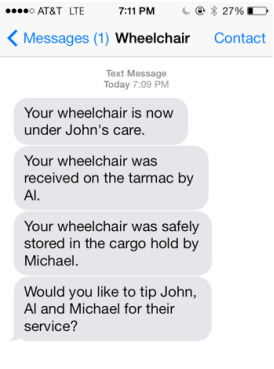
\includegraphics[width=7cm]{images/tips.png}
   \caption{One possible minimal interface for user interaction with the tracking system.}
  \label{fig:tips}
\end{figure}


\subsection{Transfer mechanism from aisle wheelchair to seat}

Once the problem of wheelchair storage storage is addressed, there is still one that needs to be solve: how do disabled passengers reach their seats once their mobility device is stored in the cargo hold? \\

Our benchmarking and interviews showed us that the transfer is one of the most demeaning moments for the handicapped, so the team focused on making the user more independent while transferring. \\

\subsubsection{Candidates}
The team agreed that the prototype should make the transfers inside the airplane so easy that the person on the aisle wheelchair could make the transfer by himself without major efforts. After a brainstorm, the team had two ideas for making this transfer: a sliding seat and a comb mechanism in which a male/female coupling system would allow the user to be transferred. The former mechanism was chosen because it was simpler to build and lighter, as it did not require a motor to lift the user or a counterweight to stabilize the chair. With that in mind, we benchmarked existing mechanisms that were used to make linear transfers. These mechanisms are listed below: \\

\noindent\emph{Linear Guide}\\
The rails would be installed on the aisle wheelchair and the seat, while the carriage would be installed on the cushion. The cushion would be able to slide from one seat to the other if the seat and the wheelchair were correctly paired.

\begin{figure}[h]
\centering
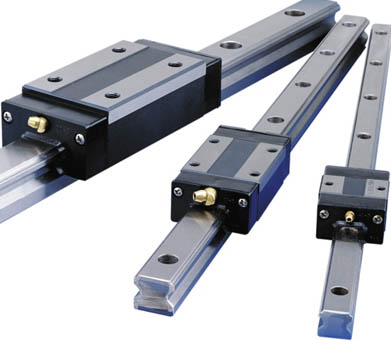
\includegraphics[width=7cm]{brazil_images/image035.jpg}
\caption{Linear guide} % - http://www.yesillerrulman.com/staf_lsk_ome_lineer_kizakli_araba_ray.html}
\label{fig:linear_guide}
\end{figure}

The negative aspect of the linear guide is that it would require a milimetric precision when pairing the aisle wheelchair with the seat. We found this to be unrealistic, especially when we took in consideration that the solution would not necessarily be automated.\\

\noindent\emph{Conveyor rollers}\\
The mechanism would use the same principles of a conveyor table, where one can move heavy objects by sliding them on top of conveyor rollers. This mechanism would be installed on the seat and the aisle wheelchair, allowing the cushion with the user to slide.

\begin{figure}[h]
\centering
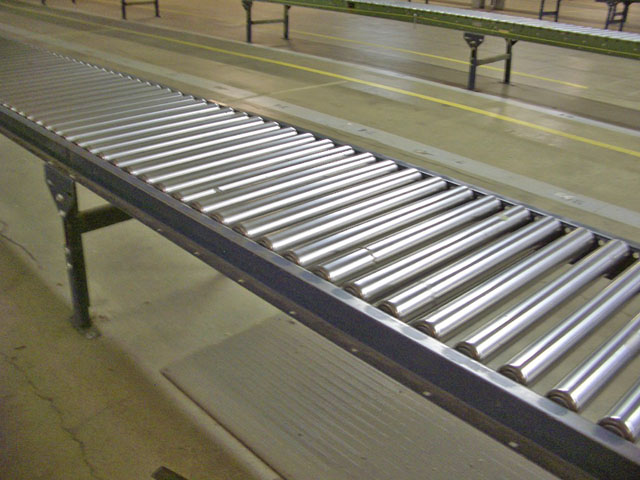
\includegraphics[width=7cm]{brazil_images/image036.jpg}
\caption{Conveyor rollers} % - http://qdtmzdhsb.cn.gongchang.com/product/d27215965.html}
\label{fig:conveyor_rollers}
\end{figure}


\noindent\emph{Caster transfer table}\\
The mechanism would work as the previous one, where the cushion would be able to slide from the aisle wheelchair to the seat, but using caster spheres instead of conveyor rollers. These spheres are lighter than the previous solution and as a result were more appropriate for our design.

\begin{figure}[h]
\centering
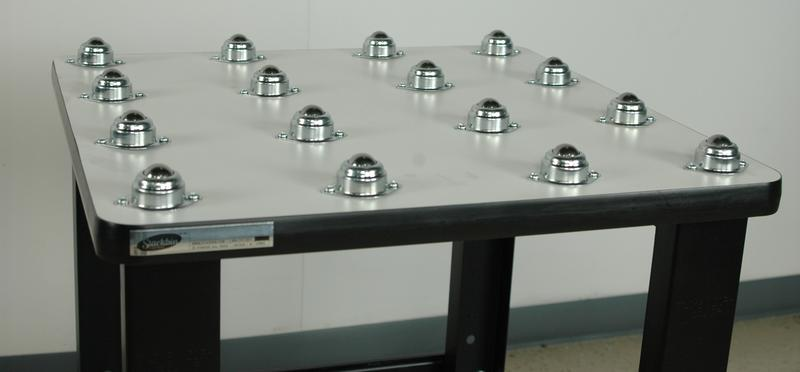
\includegraphics[width=7cm]{brazil_images/image037.jpg}
\caption{Ball transfer table}% -  http://www.stackbin.com/categories/ball-transfer-tables/ }
\label{fig:ball_transfer}
\end{figure}

Unfortunately, for our first prototype, we could not find a supplier that could provide the components in time to build the prototype with an affordable cost, so the mechanism with they conveyor roller was chosen. For the final prototype, the team was finally able to get the caster spheres into the device and implement them.

Based on what was discussed above, for the first version, the team decided to implement the seat with conveyor rollers to enable the sliding movement of the seat (Figure \ref{fig:idea_mechanism}). With the same mechanism installed on the aisle wheelchair, one would be able to easily transfer oneself laterally from the aisle wheelchair to the seat and vice versa without major efforts.

\begin{figure}[h]
\centering
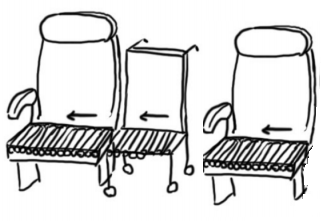
\includegraphics[width=7cm]{brazil_images/image038.png}
\caption{Idea of the mechanism}
\label{fig:idea_mechanism}
\end{figure}


\subsubsection{Building our prototype}
In our first attempt to build the prototype (Figure \ref{fig:first_attempt}) the high friction made the sliding movement extremely difficult. The main reason for this failure was that we incorrectly assumed that the aluminum cylinder directly attached to the wooden structure would be enough to make the rolling movement. \\

\begin{figure}[h]
\centering
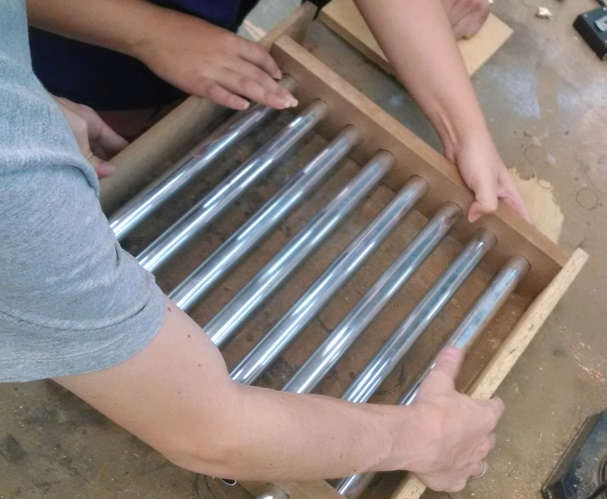
\includegraphics[width=7cm]{brazil_images/image039.jpg}
\caption{First building attempt}
\label{fig:first_attempt}
\end{figure}


In order to overcome this issue, we added bearings to both ends of the cylinders (Figure \ref{fig:fixing_bearings}). This solved the friction problem, making the whole mechanism work as we had designed it (Figure \ref{fig:final_mechanism}).	


\begin{figure}[h]
\centering
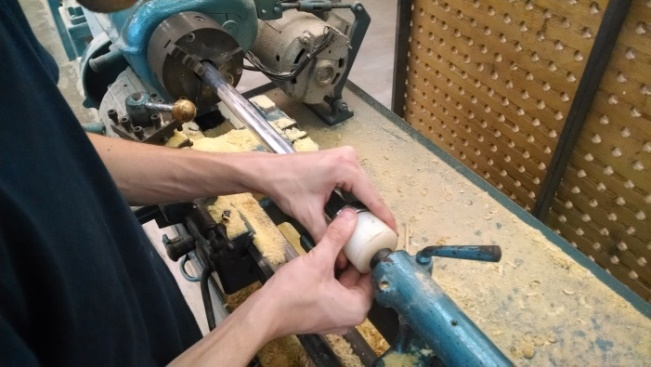
\includegraphics[width=7cm]{brazil_images/image040.jpg}
\caption{Fixing bearings}
\label{fig:fixing_bearings}
\end{figure}


\begin{figure}[h]
\centering
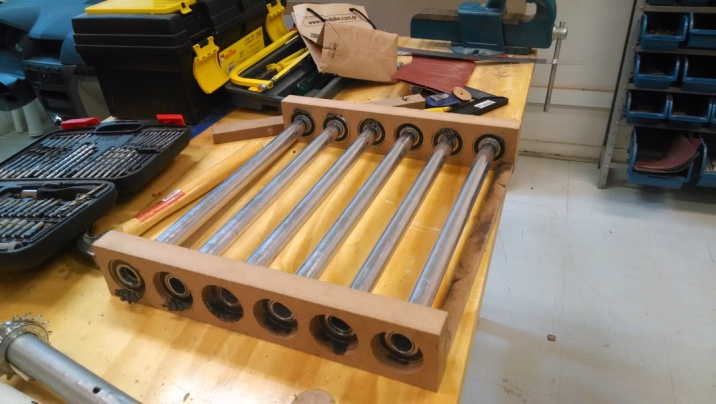
\includegraphics[width=7cm]{brazil_images/image042.jpg}
\caption{Final mechanism}
\label{fig:final_mechanism}
\end{figure}

Next, we tested the sliding mechanism with different types of materials on the cushions base. First we tried adding an adherent surface (rubber) to see how the mechanism would slide. We noticed that it was quite hard to overcome the static friction. Afterwards we tried adding a semi-rigid plastic base. Although the transfer was quite easy, one could feel the cylinders while sliding. As a result, we chose to use a hard flat base under the cushion to make it slide smoothly.   \\


\subsubsection{Learnings}

We tested our mechanism with a number of able-bodied users as we were not yet confident that it was safe enough for a disabled person to use it. We learned alot from these testing sessions and it thanks to these learnings that we were able to create a product that could be safely used by a disabled person.

\begin{itemize}
	\item The friction between the aluminum cylinder and the wood is too intense for a user to transfer from one seat to another.
	\item The space between the cushion and the mechanism must be considered to avoid increasing the friction and the looseness of the cushion (due to a rotating movement).
	\item Cushion must be firm enough so that the user does not feel the cylinders and to allow proper transfer.
	\item Correct alignment between the aisle chair and the seat is very important.
	\item Armrest must be retractable.
	\item It is possible, quite easy and comfortable to make a lateral transfer.
	\item Understanding how the mechanism will be used is crucial for achieving a user-friendly design. For instance, by simulating how a transfer would be made by an user, we noticed that it made sense to link the latching mechanism with the movement of the armrest. Armrest up, seat unlocked and vice-versa. We had several options for locking the seat, but we insisted in finding one that would be intuitive for the user. This proved to be a good design choice until we realized that users may sometimes want to put the armrest up  to get comfortably in their seats and not just because they want to transfer.
	\item Our conveyor rolling mechanism is not viable because it required too many alterations of the airplane and added too much weight.
\end{itemize}

\section{Our vision for the final product}

From all the prototypes our team built during winter quarter we decided to combine the two products: the wheelchair platform and the transfer mechanism into one single enhanced experience for passengers with reduced mobility. \\

Figure \ref{fig:our_vision} shows the different steps our user should go through in order to get a much better flying experience than what they have today. \\


\begin{figure}[h]
  \centering
     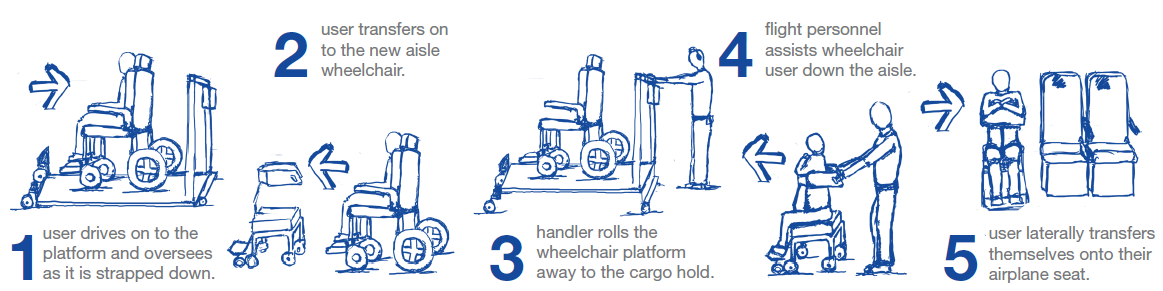
\includegraphics[width=16cm]{images/our_vision.png}
   \caption{Our vision for the final product}
  \label{fig:our_vision}
\end{figure}

In order to include the two products (wheelchair platform and transfer mechanism) into the one single experience for the passengers, we realized that our team would also have to completely redesign the aisle wheelchair to enable a smooth transfer from the passenger’s wheelchair to the airplane seat.\\


With this vision in mind, our objective for the spring quarter was to build and test with users:
\begin{itemize}
\item The wheelchair platform
\item The redesigned aisle wheelchair
\item The transfer mechanism integrated into an airplane seat
\end{itemize}

All the design requirements associated with these products are presented in the next section and the design specification section gives many details about the design solutions we implemented for each system.\\

Unfortunately, due to time constraints, we did not get th opportunity to develop and create a smartphone app that would provide wheelchair users with information about their trip and the way their mobility device is handled by the airline. We instead decided to focus more on the hardware than the software but additional information about what we envisioned for the app can be found in Appendix G.